
\chapter{Block recognition}\label{ch:block_recognition}

The block recognition part has been divided into 5 main steps: 
\begin{itemize}
  \item background substraction
  \item color detection
  \item edge detection
  \item position
  \item orientation
\end{itemize}

\section{Background substraction}
As a first step a background substraction was performed, such that the gray area around the blocks is neglected and a proper color detection is applied. Also, this deals with the uneven illumination in the images which results in smoother edges. 

This is done by substracting the 2D median filtered image from the initial one as in Equation \ref{eq:rem_alg}. In the case of the white block, the background substraction partially erases the block's shape. However, it will be reconstructed later in the edge detection stage. 

\begin{equation}\label{eq:rem_alg}
  \begin{cases}
    Image(x,y) = I(x,y) - \overline{I(x,y)} \\
    \overline{I(x,y)} = medfilt2(I(x,y))
  \end{cases}
\end{equation}

\begin{figure}[H]
  \centering
  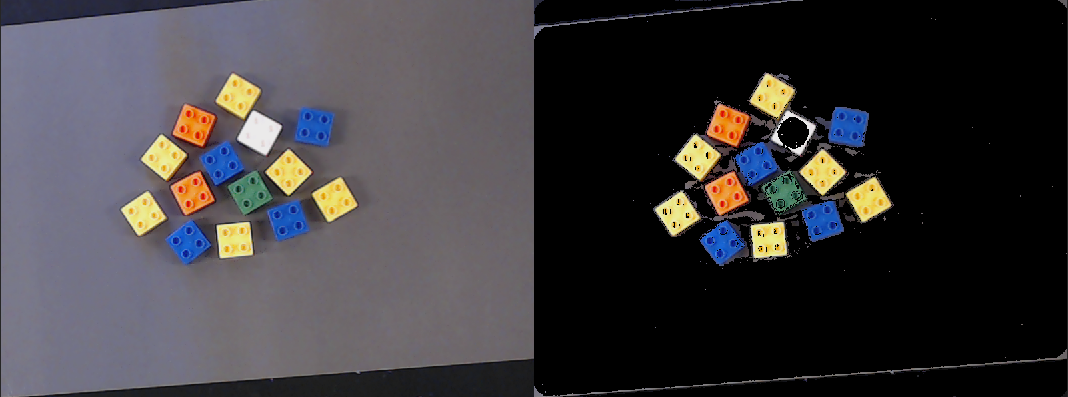
\includegraphics[scale=0.35]{figures/remove_background.png}
  \caption{Camera image with background substracted}
  \label{fig:rem_back}
\end{figure}

\section{Color detection}

 	Once the background is substracted, the color of the blocks is experimentally obtained by using the tool \textit{Pixel region} in MATLAB. A color can be described with values between 0 and 255 for its primary colors, red, green and blue. Thus, for each block, the \textit{Pixel region} tool has been placed on it to get a range for the RGB parameters.\par

An example with the yellow block is given below
\par

\begin{figure}[hb]
  \centering
  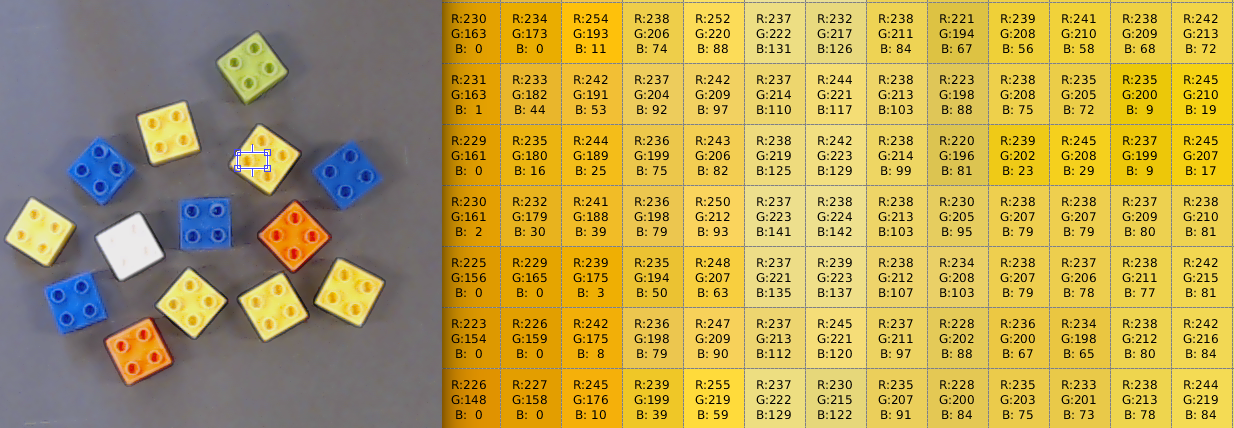
\includegraphics[scale=0.3]{figures/Thres_Y_manualy2.png}
  \caption[LABEL] {RGB selection}
  \label{fig:color1}
\end{figure}

Figure \ref{fig:color1} gives us more or less a range for the RGB parameters. These parameters are then used to check in a loop (thresholding) that every pixel of the image are within the ranges.\par
%In the image below the pixels being in the RGB parameter are highlighted in white while the others are put into black. 

\begin{figure}[hb]
  \centering
  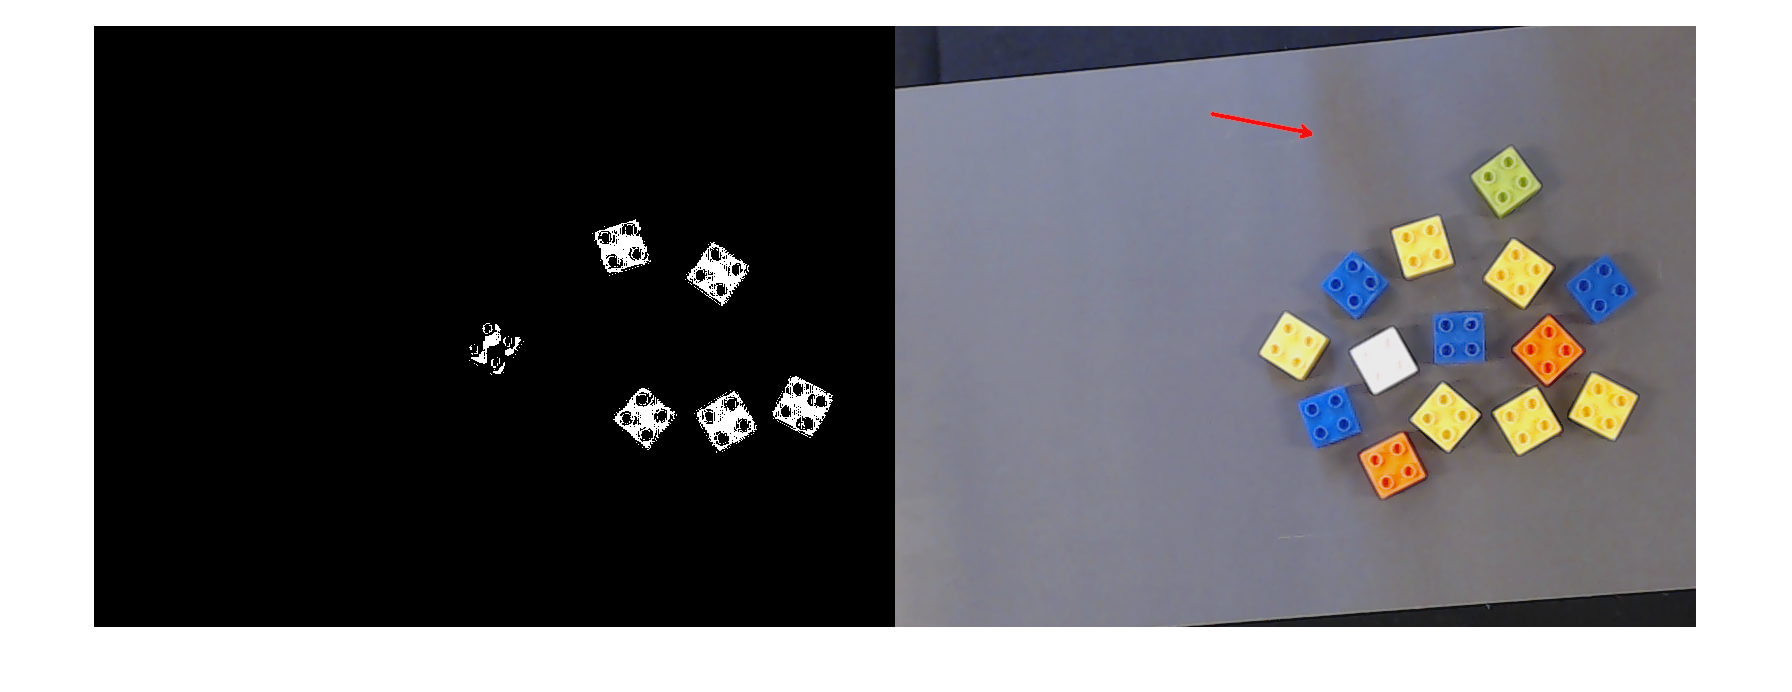
\includegraphics[scale=0.3]{figures/Thres_Y_bad2.png}
  \caption[LABEL] {First attempt color thresholding}
  \label{fig:color2}
\end{figure}
  

In figure \ref{fig:color2}, the 6 yellow blocks are detected. However, the one on the left is partially detected. This is the consequence of the different lightings in the robot cell. The RBG range was defined on a block placed in a zone of shadow (see the red arrow on the picture). \par


Thus, the color recognition was redefined taking into account the different lightings inside the robot cell. All the yellow blocks are now detected.



\begin{figure}[H]
  \centering
  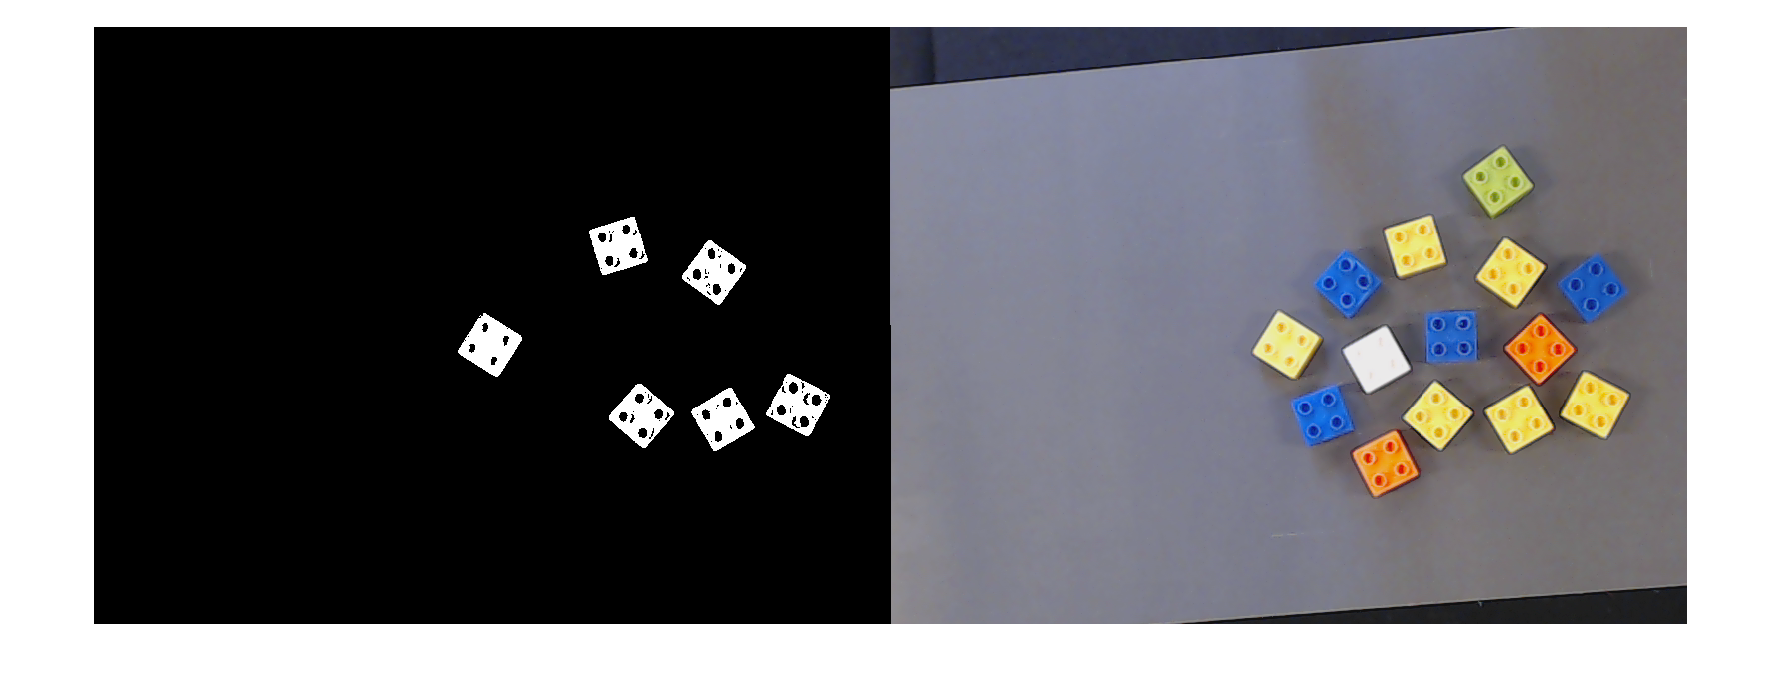
\includegraphics[scale=0.3]{figures/Thres_Y_good.png}
  \caption[LABEL] {Correct color thresholding}
\end{figure}

An other solution would have been to set up a constant lighting inside the cell to have more precise ranges for the colors, resulting in a more robust system.



 \section{Edge detection}

	There are different methods to detect the edges in an image. To pick the best one for this application, different methods such as the Canny, log, Prewitt, Roberts, Sobel and zerocross were tested along with their parameters, the threshold, direction and the standard deviation of the filter. \par


	The detection of the edges was based on the resulting image of the color recognition. Below can be seen the color recognition of the blue blocks.

	\begin{figure}[H]
  \centering
  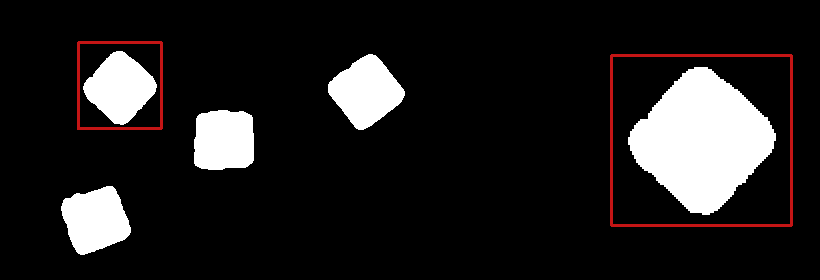
\includegraphics[scale=0.3]{figures/color_rec_zoom.png}
  \caption[LABEL] {Post color recognition step}
\end{figure}	
	


As seen on the picture above, the shapes of the blocks that resulted from the color recognition step are irregular and so are be the edges. Thus, we used the Canny method that allows us to choose a stantard deviation of its filter in order to smooth the irregularities of the shapes.\par 



The default value of the deviation is $\sqrt{2}$, increasing the deviation will result in smoother lines until getting a round shape.

\begin{figure}[H]
\hfill
\subfigure[Canny default]{
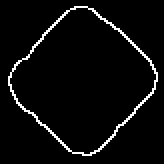
\includegraphics[scale=0.5]{figures/Canny_sqrt2.png}
\label{fig:subim11}}
\hfill
\subfigure[Canny 4]{
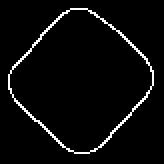
\includegraphics[scale=0.5]{figures/Canny_4.png}
\label{fig:subim12}}
\hfill
\subfigure[Canny 10]{
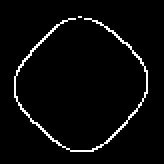
\includegraphics[scale=0.5]{figures/Canny_10.png}
\label{fig:subim12}}
\hfill
\subfigure[Canny 25]{
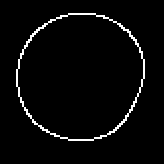
\includegraphics[scale=0.5]{figures/Canny_25.png}
\label{fig:subim12}}
\hfill

\caption{Canny edge detection method}

\end{figure}

As a result of the tests done, the Canny method with a standard deviation of 4 was the one chosen, giving us smoother lines but not too round corners in order to calculate its position.



 \section{Position and Orientation}\label{ch:position_rotation}

As it has been shown before, once the threshold segmentation has been applied to our cropped image from the workspace, the picture will look something of this sort:

\begin{figure}[hb]
  \centering
  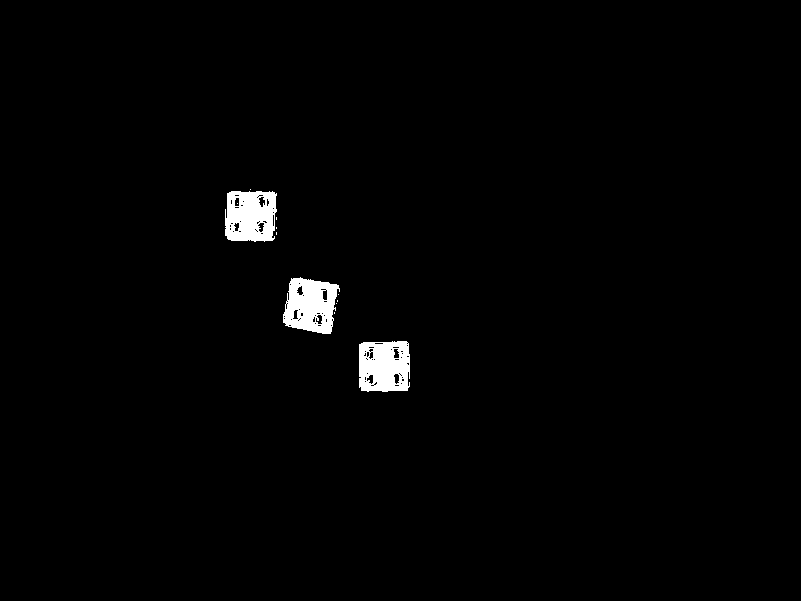
\includegraphics[scale=0.3]{figures/thresh_img.png}
  \caption[thresholded_image] {RGB Segmented Image}
\end{figure}

\subsection*{Position}
The goal of this project is to try to pick the bricks, creating Simpson characters with them. Therefore, it is imperative to have a precise position of every block in order to be able to give the correct coordinates to the gripper. This is the reason why the position becomes one of the most important steps in this project.

After computing the picture taken by the camera, the detection of the center involved the creation of areas that would be labeled. Hence, it was necessary to detect the edges of the bricks in order to find their squared shapes and, then, the square was filled, creating an homogeneous area.

Finally, \textit{Regionprops} function was used to detect the center of each white area (binary image). The detected center was the center of mass and not the geometrical one, however, the differences between them were very small because the area was homogeneously filled.


\subsection*{Orientation}
Besides the position, the measure of the required angle to turn the gripper is also essential to achieve the goal. Nevertheless, the coordinates of the center will be important to find the orientation of the bricks. 

First, four furthest points with respect to the center are necessary to find the coordinates of the corners. However, this search needs to be constrainted to ensure that the distance between each point is, at least, fifteen pixels, to avoid having more than one point in each corner.

Then, two of the previous corners are chosen in order to define one side of the square. The connection between these two corners and the center generates two different straight lines (from each corner to the center). Using the image with the edges of the desired block it was evaluated which points were below the generated lines. To finish this step, a linear regression was calculated and the parameters of the straight line were found.

\begin{figure}[hb]
\hfill
\subfigure[Straight lines that connect the corners with the center of the brick]{
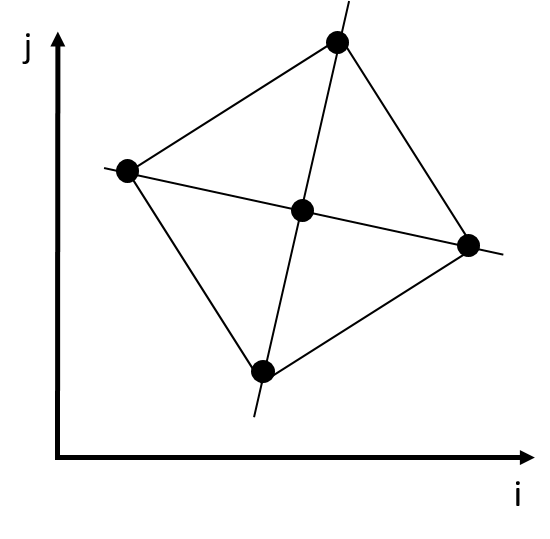
\includegraphics[scale=0.5]{figures/diag_square.png}
\label{fig:subim11}}
\hfill
\subfigure[Side of the square used for calculating the slope]{
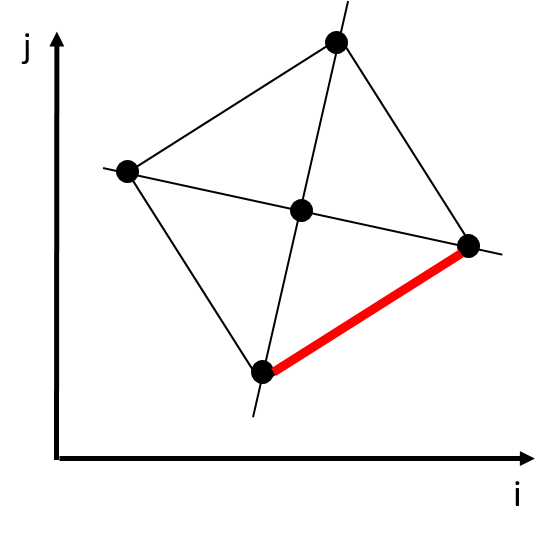
\includegraphics[scale=0.5]{figures/diag_square_side.png}
\label{fig:subim12}}
\hfill
\caption{Brick in the world frame}
\end{figure}

Finally, the slope was converted to an angle to obtain the orientation of the brick. However, if the angle was negative it was necessary to calculate the one associated with the perpendicular line in order to have the correct orientation.

\begin{figure}[hb]
\hfill
\subfigure[Positive slope - it gives directly the orientation]{
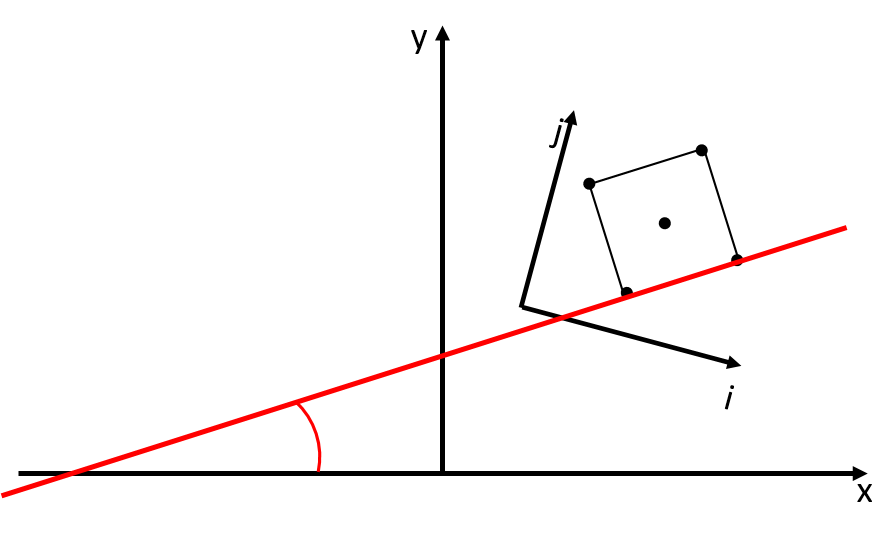
\includegraphics[scale=0.45]{figures/posit_slope.png}
\centering
\label{fig:subim21}}
\hfill
\subfigure[Negative slope - it gives indirectly the orientation]{
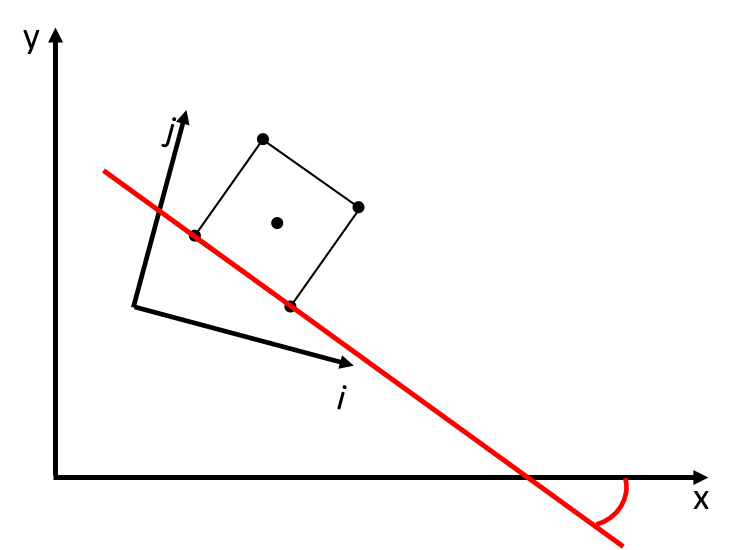
\includegraphics[scale=0.45]{figures/neg_slope.png}
\label{fig:subim22}}
\hfill
\caption{Orientation of the brick in the robot frame}
\label{fig:image2}
\end{figure}